
% Experement data + calcs goes here %

\section{Ход работы}

\subsection{Измерение характеристик контура для разных емкостей}

Произвел измерение характеристик контура для разных емкостей (см листочек с данными).

\noindentИз данных получаю значение индуктивности катушки: \mth{L = 993,7} мкГн.
\noindentИз данных получаю значения добротности: \mth{Q_3 = 20,13}; \mth{Q_6 = 14,35}.

\subsection{Измерение АЧХ для разных емкостей}

Произвел измерение АЧХ для 2 разных емкостей (снял много точек для C3 и три - для C6). Результаты измерений присутствуют на листочке с данными. График для C3 представлен на рисунке 2.

\begin{center}

    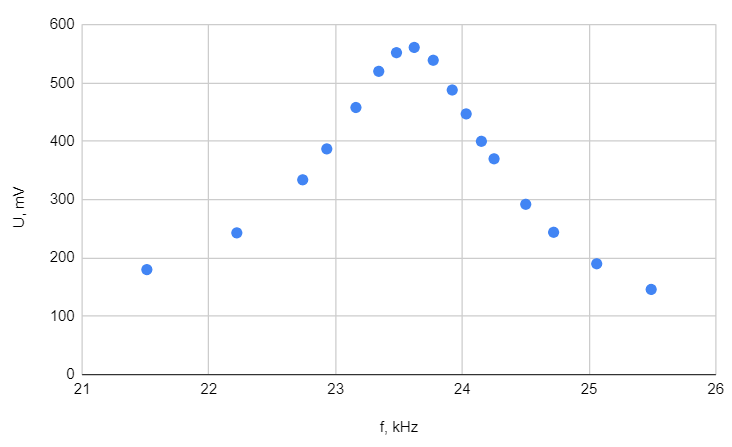
\includegraphics[scale=0.9]{picks/323-graph1.png} \\
    \textit{Рис. 2. АЧХ}

\end{center}

\noindentЗначения добротности для C6 и С3: \mth{Q_3 = 19,42}; \mth{Q_6 = 13,92}. Полученные значения отличаются в \mth{\approx} 1.4142 раза, что согласуется с теоретической формулой. Так же полученные значения совпали с значениями, полученными в п.1.

\newpage

\subsection{Измерение ФЧХ}

Произвел измерение ФЧХ для емкости C3. График представлен на рисунке 3.

\begin{center}

    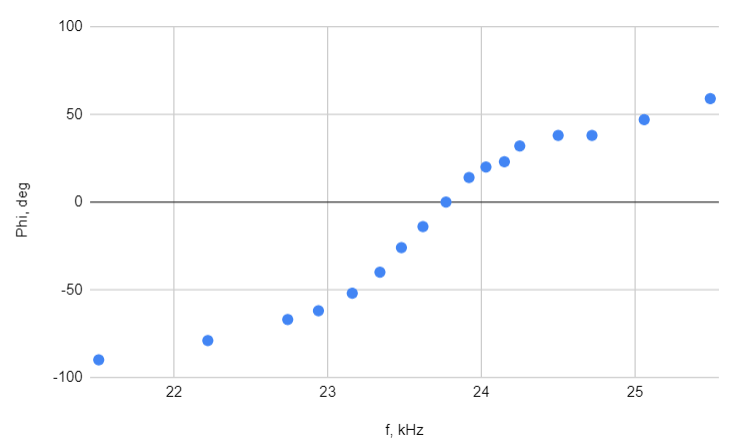
\includegraphics[scale=0.9]{picks/323-graph2.png} \\
    \textit{Рис. 3. ФЧХ}

\end{center}

\noindentПосчитал добротность по ФЧХ: \mth{Q = \frac{1}{\Delta f}}, где \mth{\Delta f} - диапозон частот, на котором угол меняется от \mth{-\frac{\pi}{4}} до \mth{+\frac{\pi}{4}}.

\noindent\mth{Q = 19,34}

\section{Вывод}

В ходе данной работы были получены ФЧХ и АЧХ для LRC контура. Видно, что зависимости совпадают с теоретическими. Также были различными способами получены значения добротности для LRC контура, данные значения совпали с хорошей точностью для различных методик подсчета.